\section{Двигатель постоянного тока}
Рассмотрим уравнения двигателя постоянного тока:
\begin{equation}
    J\dot{\omega} = M,\quad M = k_mI,\quad I=\frac{U + \varepsilon_i}{R},\quad\varepsilon_i = -k_e\omega
\end{equation}
Составим с их помощью модель двигателя постоянного тока:
\begin{equation}
    \dot{\omega} + \frac{k_ek_m}{JR}\omega = \frac{k_m}{JR} U
    \label{eq:dc_motor_deq}
\end{equation}
Запишем в виде передаточной функции:
\begin{equation}
    W(s) = \frac{k_m}{JRs + k_ek_m}
    \label{eq:dc_motor_tf}
\end{equation}
Получаем апериодическое звено первого порядка:
\begin{equation}
    W(s) = \frac{\frac{1}{k_e}}{Ts + 1}, \quad T = \frac{JR}{k_ek_m}
\end{equation}
\subsection{Временные характеристики}
\noindent Найдем весовую функцию системы:
\begin{equation}
    y_{\text{i.r.}}(t) = L^{-1}\left\{\frac{1}{Ts + 1}\cdot\frac{1}{k_e}\right\} = \frac{1}{Tk_e}e^{-\dfrac{t}{T}} 
\end{equation}
Найдем переходную функцию:
\begin{equation}
    y_{\text{s.r.}}(t) = L^{-1}\left\{\frac{1}{Ts + 1}\cdot\frac{1}{k_e}\cdot\frac{1}{s}\right\} = \frac{1}{k_e} \left(1 - e^{-\dfrac{t}{T}}\right)
\end{equation}

Построим графики весовой (см. рис. \ref{fig:task1_impulse_response_eq}) и переходной (см. рис. \ref{fig:task1_step_response_eq}) функций.
\begin{figure}[ht!]
    \centering
    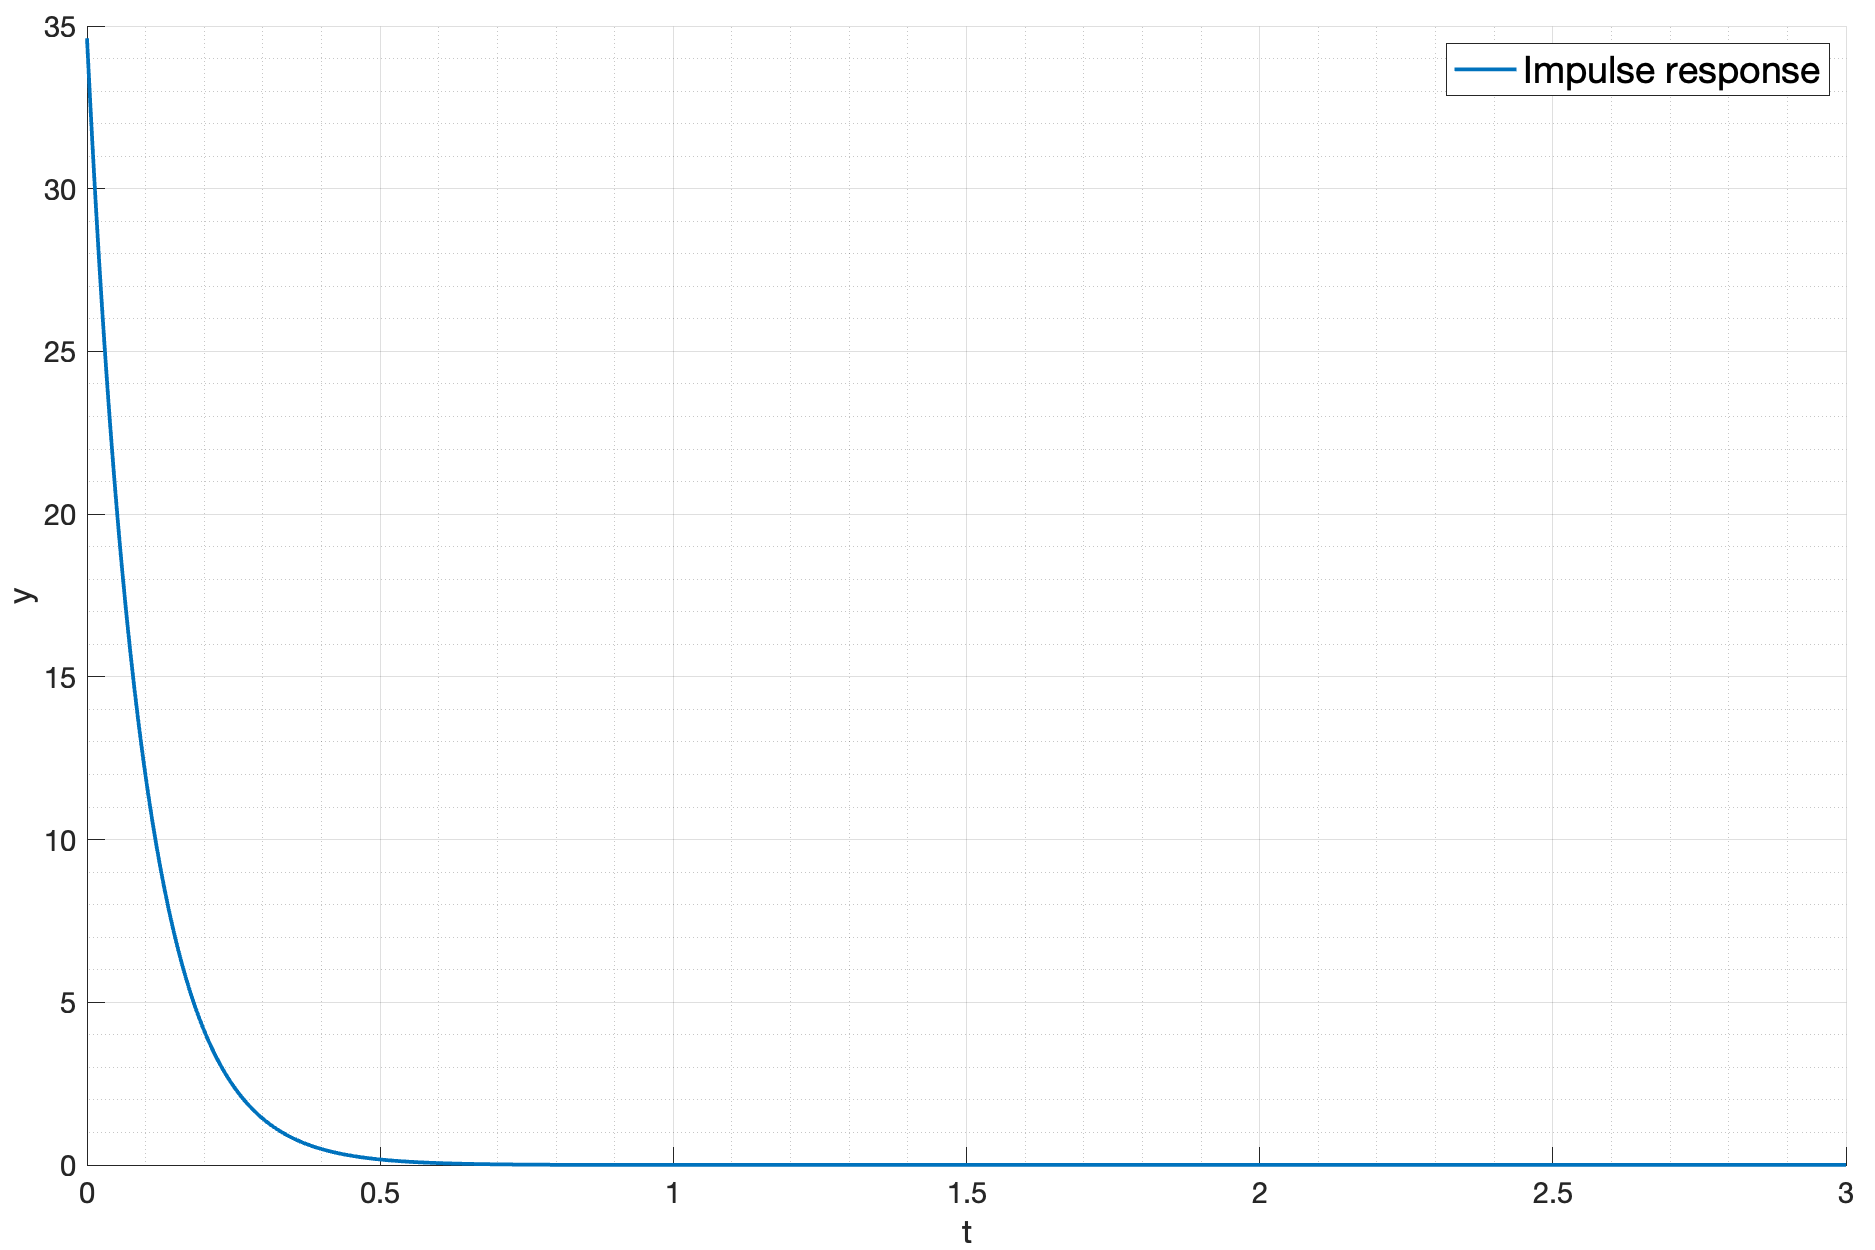
\includegraphics[width=\textwidth]{media/plots/task1_impulse_response_eq.png}
    \caption{Весовая функция двигателя постоянного тока (теоретически)}
    \label{fig:task1_impulse_response_eq}
\end{figure}
\begin{figure}[ht!]
    \centering
    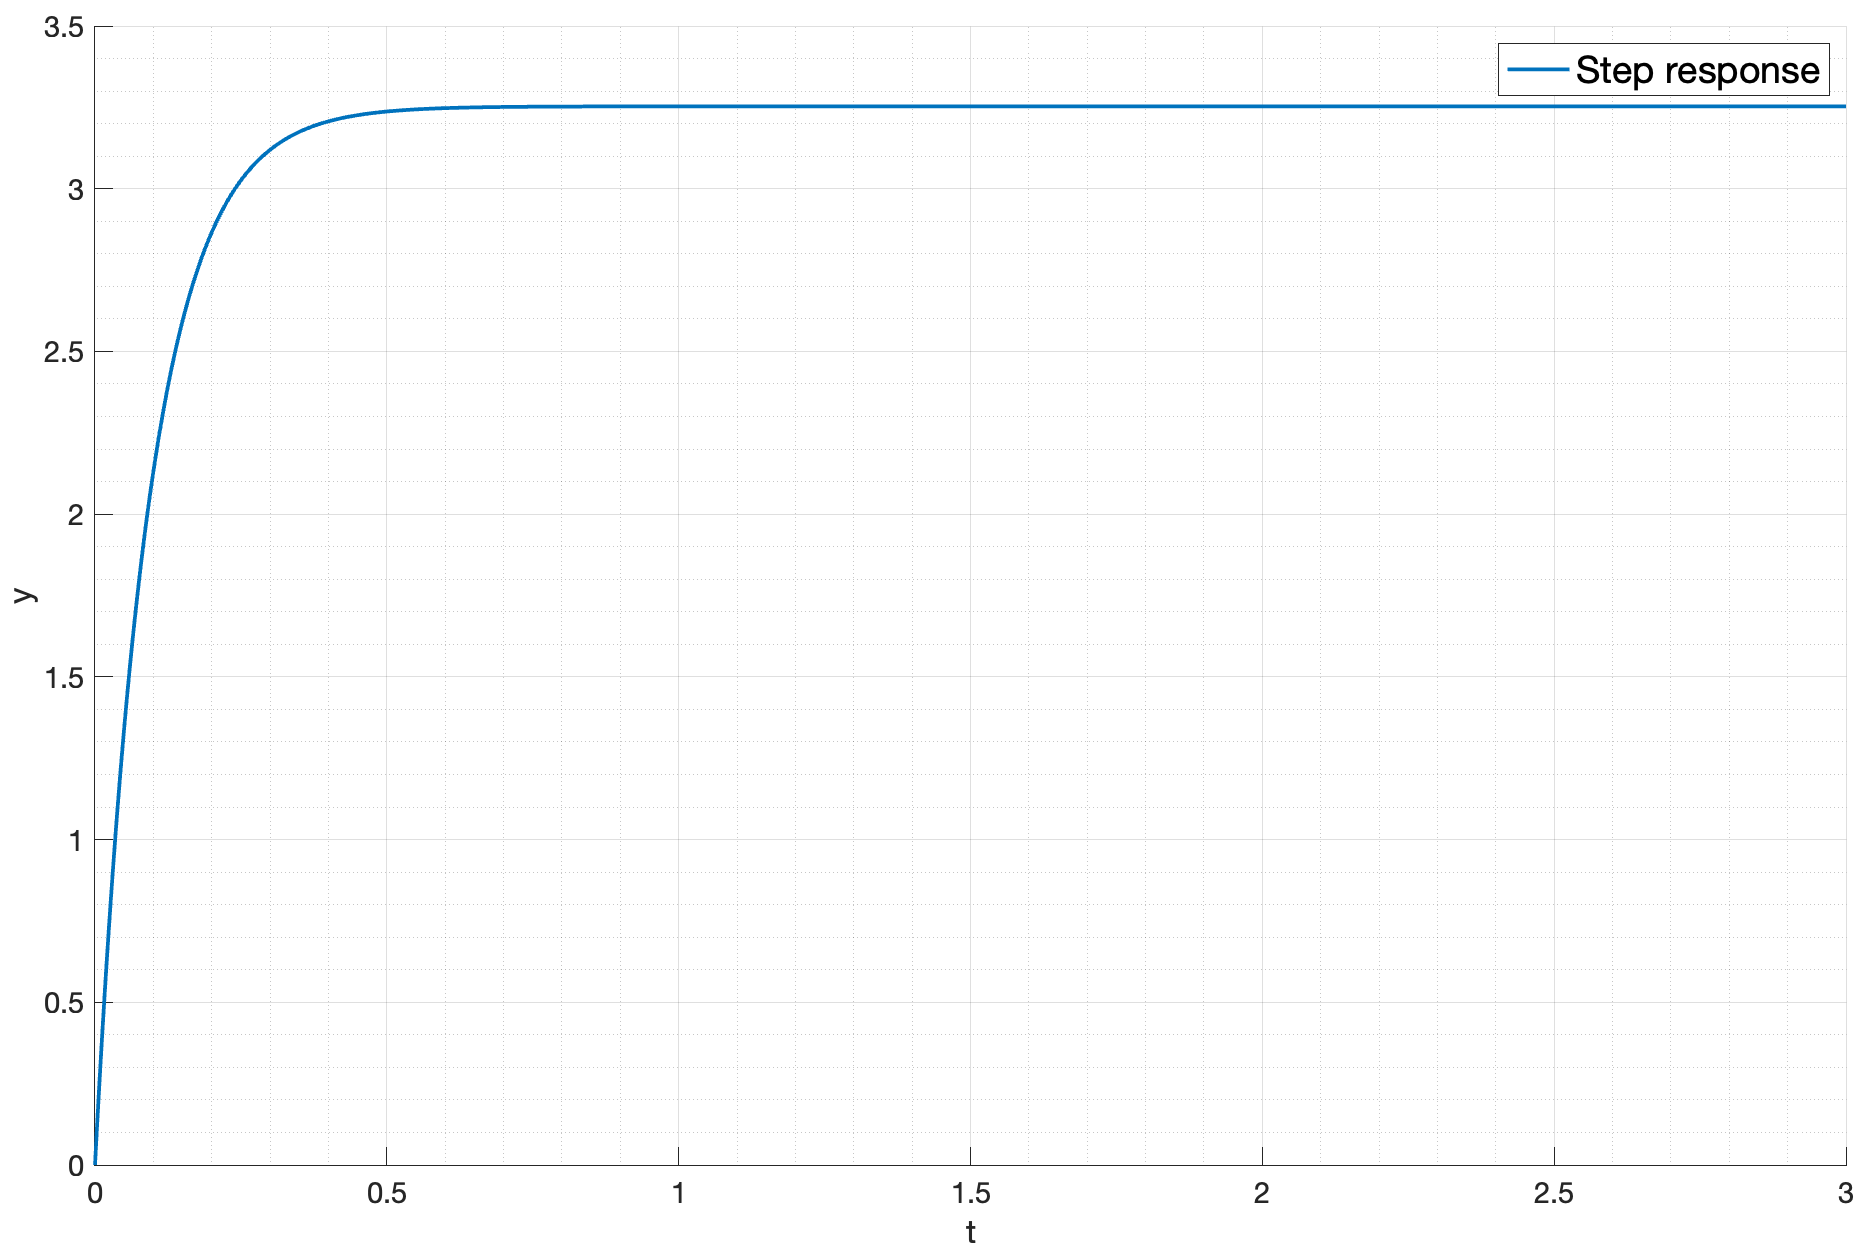
\includegraphics[width=\textwidth]{media/plots/task1_step_response_eq.png}
    \caption{Переходная функция двигателя постоянного тока (теоретически)}
    \label{fig:task1_step_response_eq}
\end{figure}

Весовая (см. рис. \ref{fig:task1_impulse_response_exp}) и переходная (см. рис. \ref{fig:task1_step_response_exp}) функции, полученные в результате моделирования: 
\begin{figure}[ht!]
    \centering
    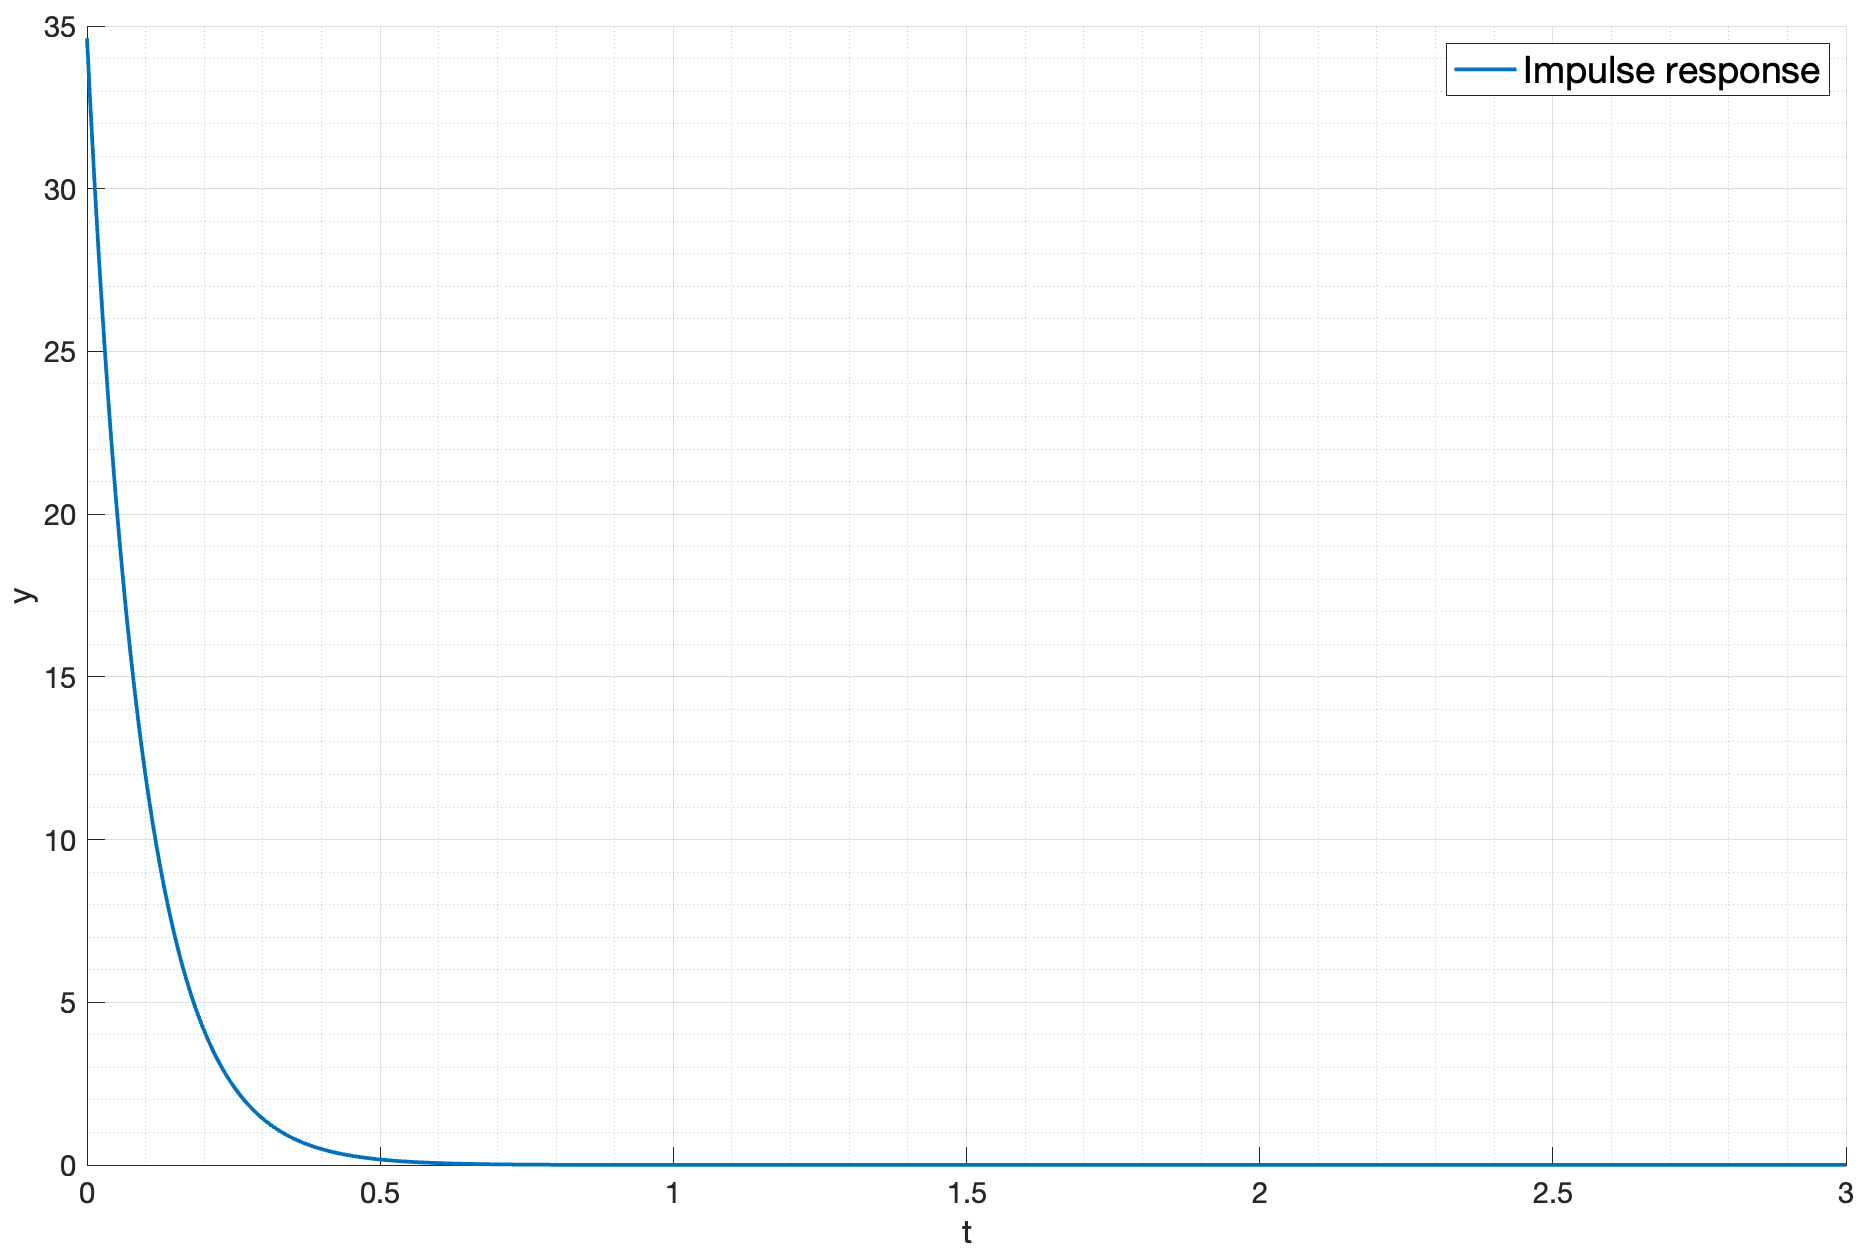
\includegraphics[width=\textwidth]{media/plots/task1_impulse_response_exp.png}
    \caption{Весовая функция двигателя постоянного тока (экспериментально)}
    \label{fig:task1_impulse_response_exp}
\end{figure}
\begin{figure}[ht!]
    \centering
    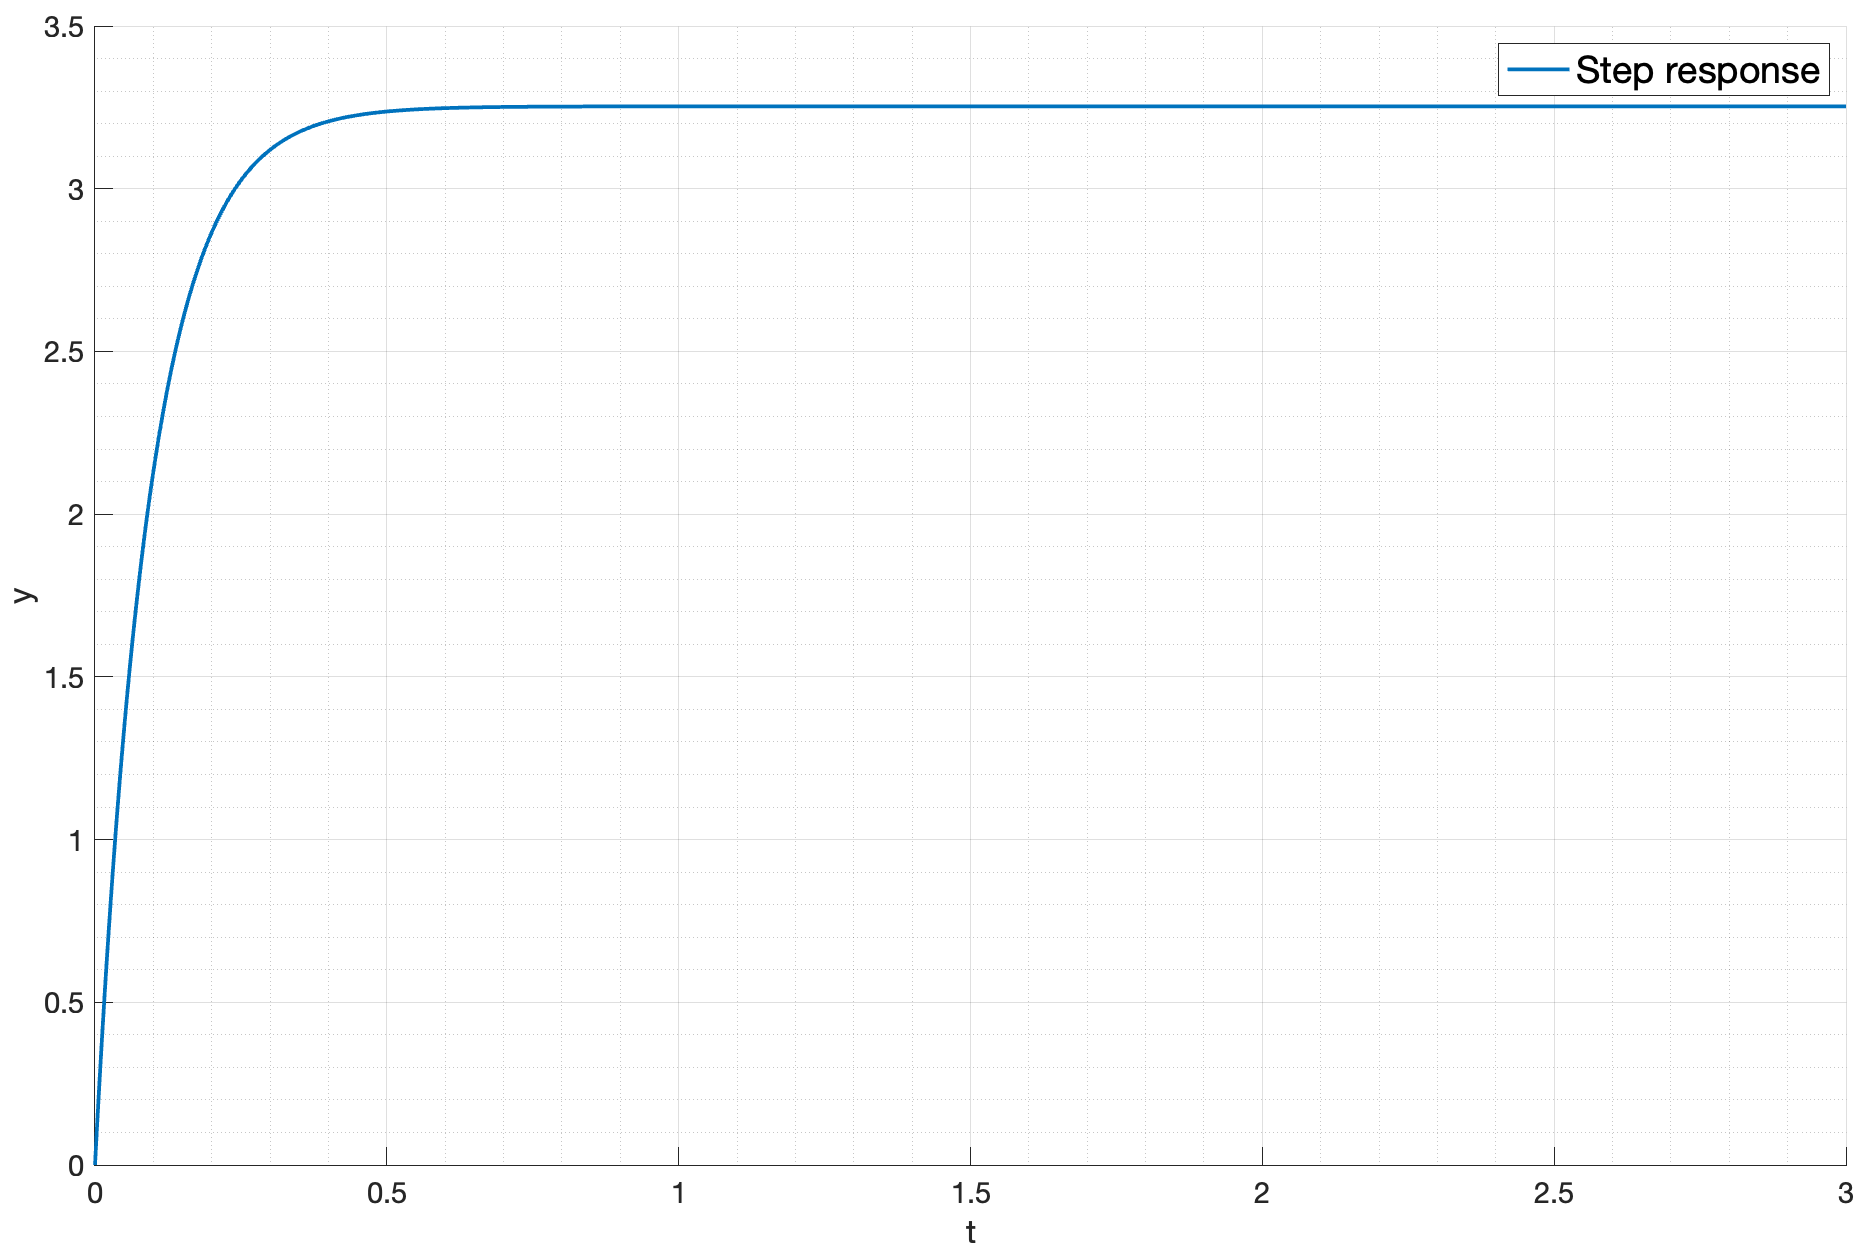
\includegraphics[width=\textwidth]{media/plots/task1_step_response_exp.png}
    \caption{Переходная функция двигателя постоянного тока (экспериментально)}
    \label{fig:task1_step_response_exp}
\end{figure}

Сравнительные графики приведены на рис. \ref{fig:task1_impulse_response_cmp} и рис. \ref{fig:task1_step_response_cmp}.
\begin{figure}[ht!]
    \centering
    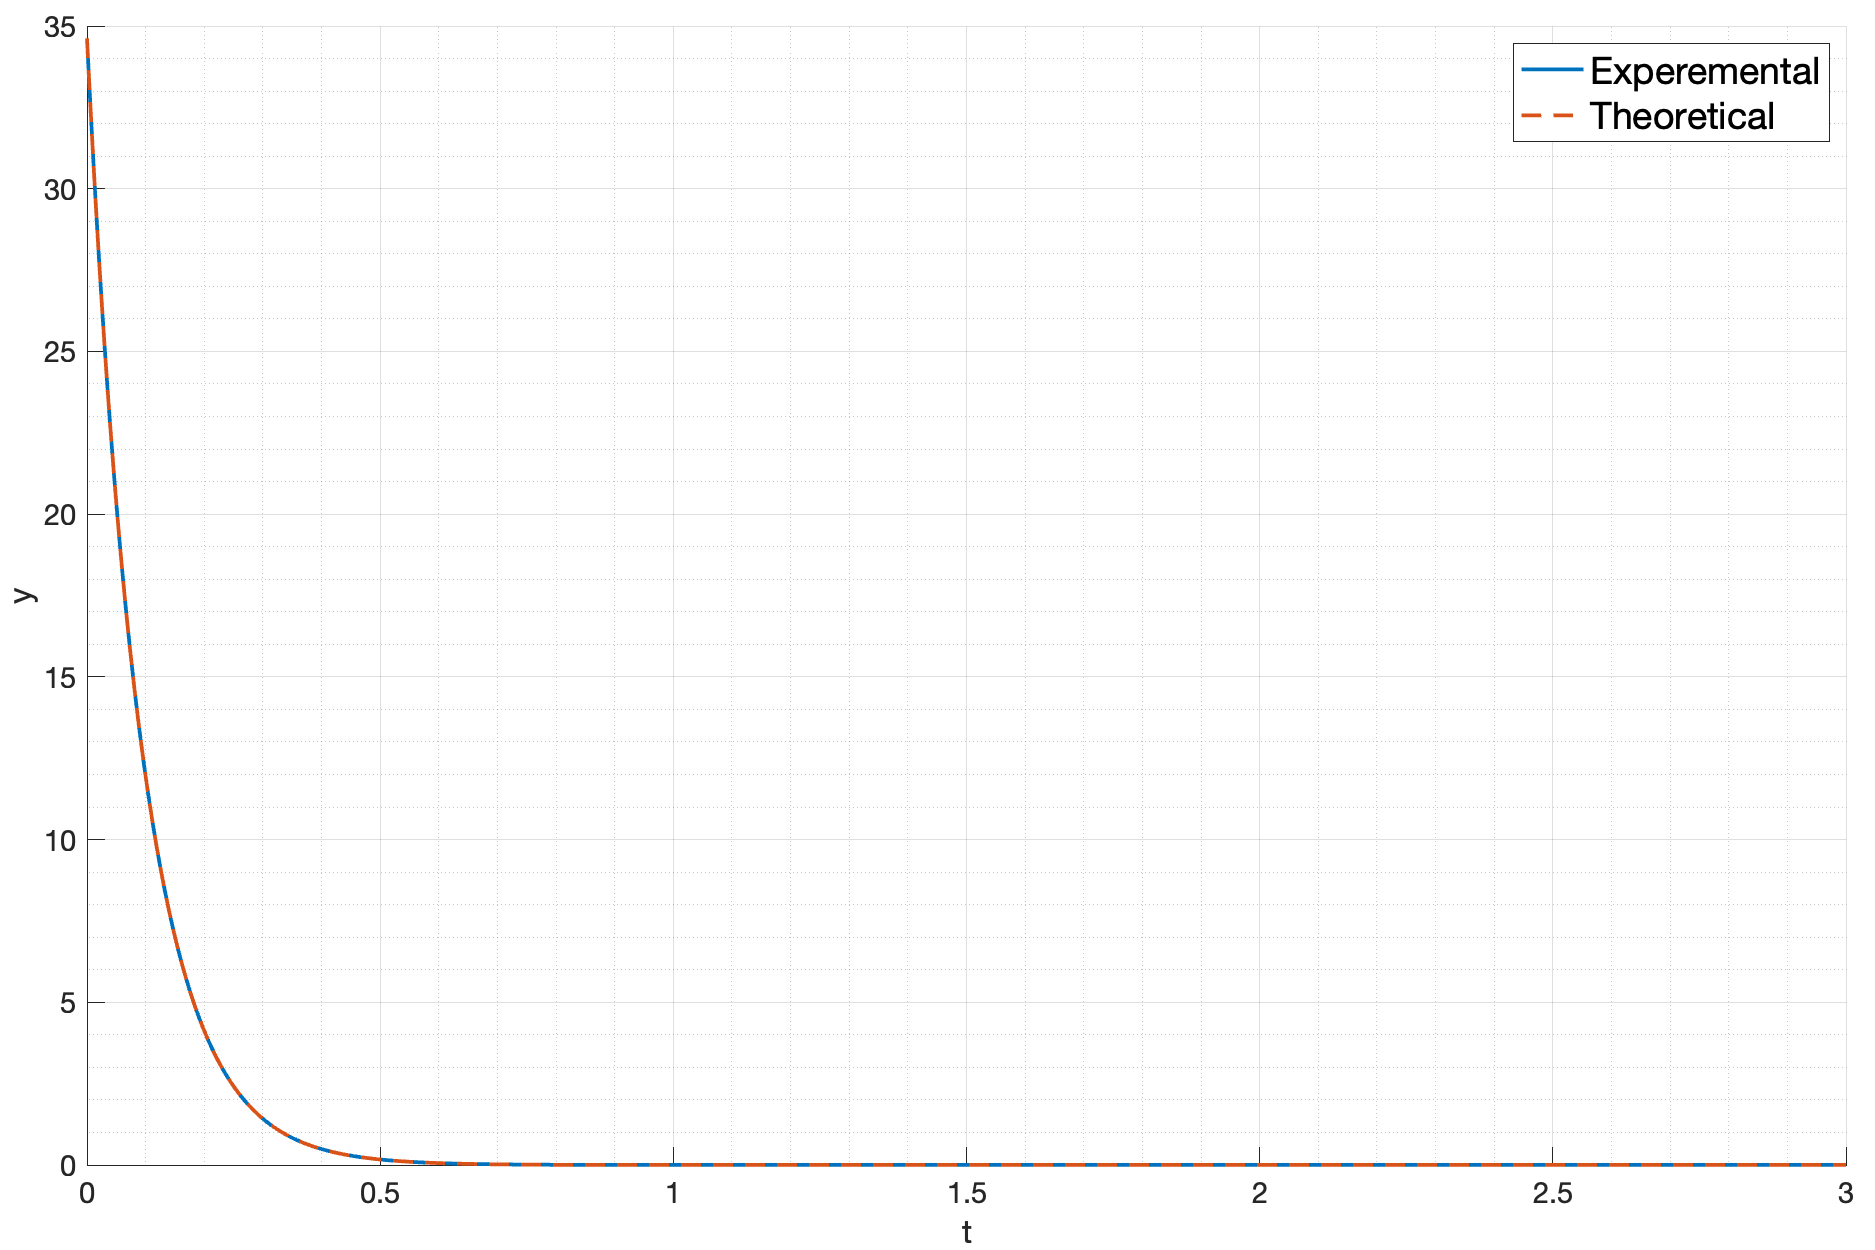
\includegraphics[width=\textwidth]{media/plots/task1_impulse_response_cmp.png}
    \caption{Сравнение весовых функций двигателя постоянного тока}
    \label{fig:task1_impulse_response_cmp}
\end{figure}
\begin{figure}[ht!]
    \centering
    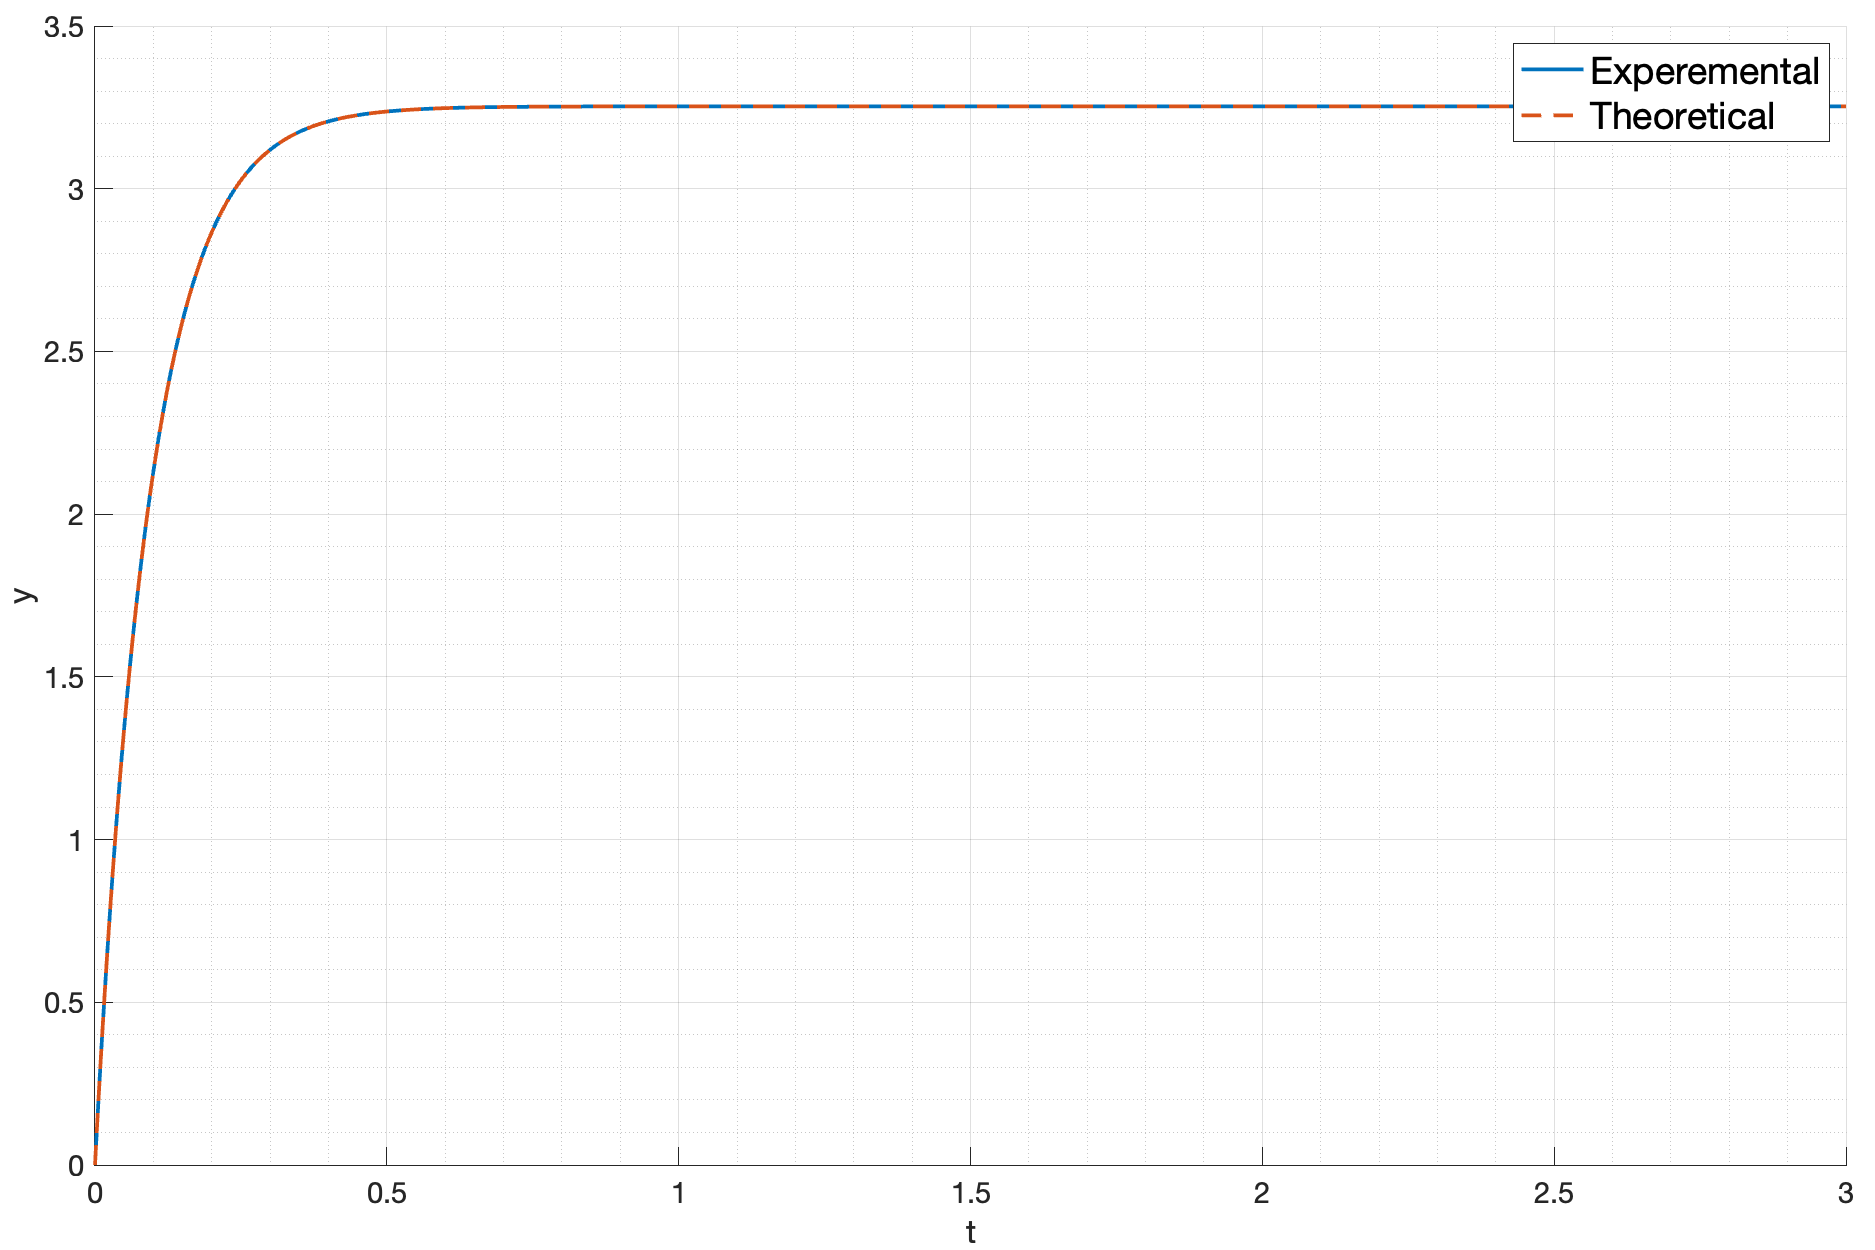
\includegraphics[width=\textwidth]{media/plots/task1_step_response_cmp.png}
    \caption{Сравнение переходных функций двигателя постоянного тока}
    \label{fig:task1_step_response_cmp}
\end{figure}

Видно, что в обоих случаях теоретические и экспериментальные графики совпадают.

\FloatBarrier
\subsection{Частотные характеристики}
\noindent Найдем амплитудно-частотную характеристику и фазо-частотную характеристику,
выделив вещественную и мнимую части частотно-передаточной функции:
\begin{equation}
    W(j\omega) = \frac{\frac{1}{k_e}}{j\omega T + 1} = \frac{1}{k_e}\frac{1}{\sqrt{\omega^2T^2 + 1}}e^{-j\arctan(\omega T)}
\end{equation}
Таким образом, АЧХ:
\begin{equation}
    A(\omega) = \frac{1}{k_e\sqrt{\omega^2T^2 + 1}}
\end{equation}
ФЧХ:
\begin{equation}
    \varphi(\omega) = -\arctan(\omega T)
\end{equation}
Найдем логарифмическую АЧХ: 
\begin{equation}
    L(\omega) = 20\lg(A) = -20\lg(k_e) - 10\lg(\omega^2T^2 + 1)
\end{equation}

Построим графики АЧХ, ФЧХ (см. рис. \ref{fig:task1_freq_resp_eq_lin}) и логарифмическую АЧХ (см. рис. \ref{fig:task1_freq_resp_eq_loglog}).
\begin{figure}[ht!]
    \centering
    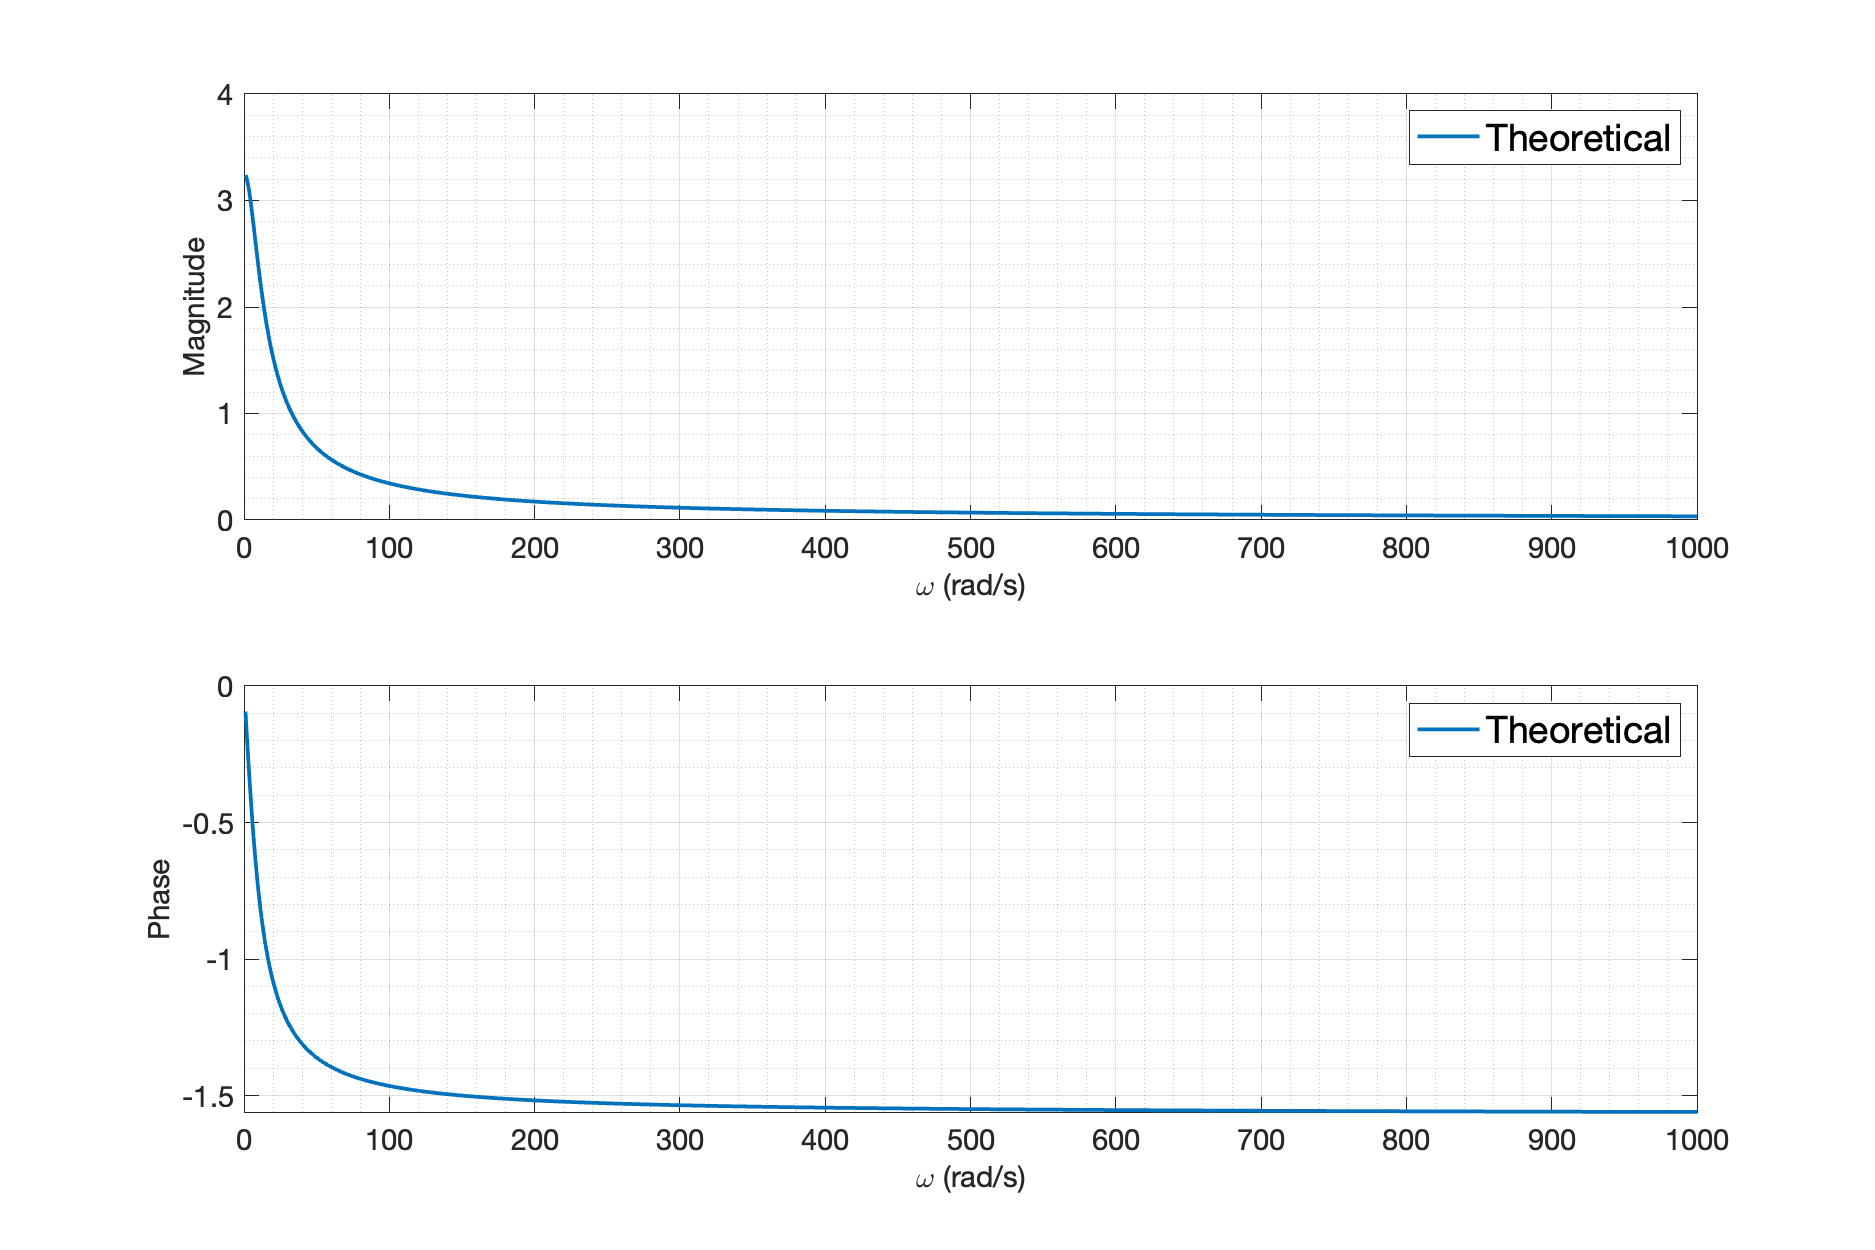
\includegraphics[width=\textwidth]{media/plots/task1_freq_resp_eq_lin.png}
    \caption{АЧХ и ФЧХ двигателя постоянного тока (теоретически)}
    \label{fig:task1_freq_resp_eq_lin}
\end{figure}
\begin{figure}[ht!]
    \centering
    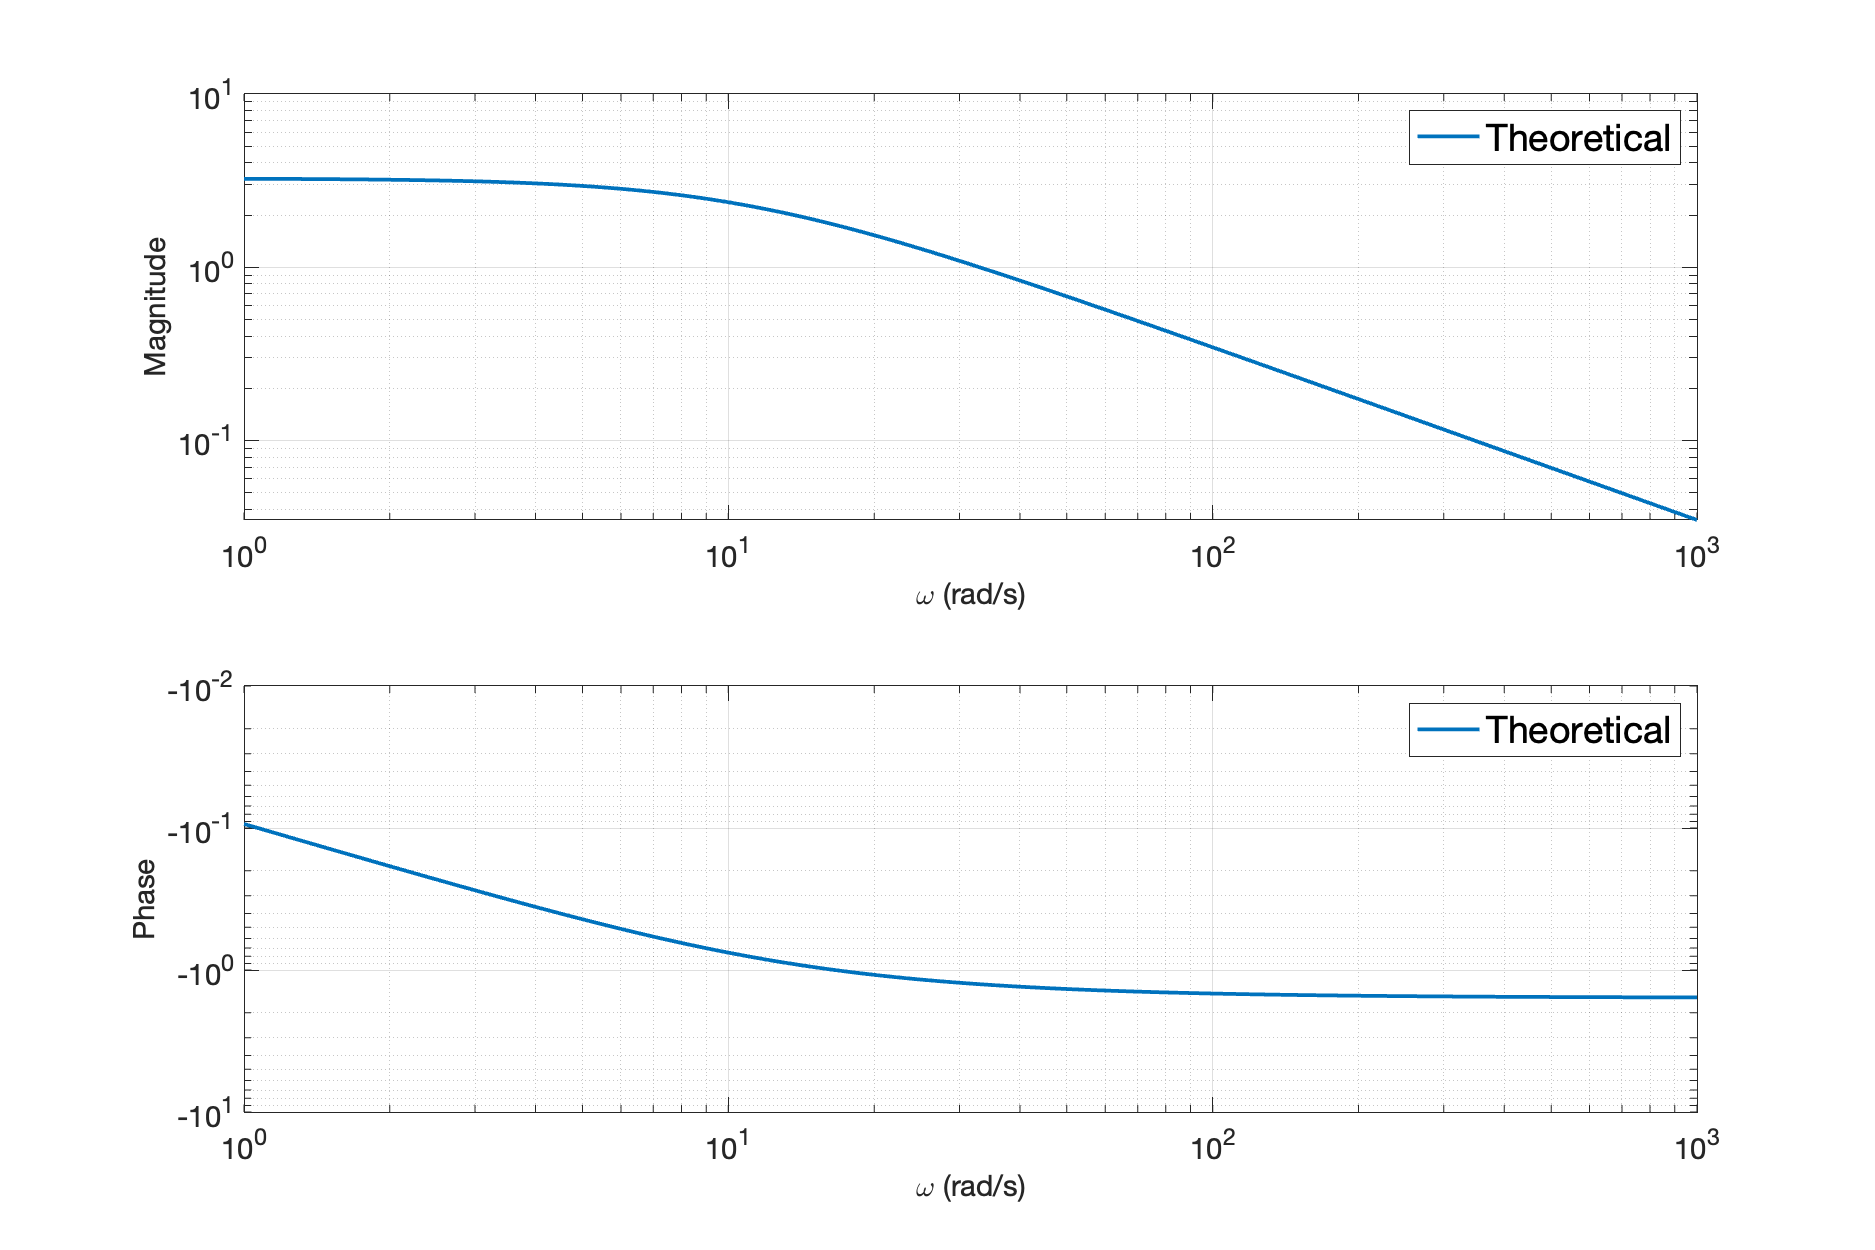
\includegraphics[width=\textwidth]{media/plots/task1_freq_resp_eq_loglog.png}
    \caption{Логарифмическая АЧХ двигателя постоянного тока (теоретически)}
    \label{fig:task1_freq_resp_eq_loglog}
\end{figure}

AXH, ФЧХ и логарифмическая АЧХ, полученные в результате моделирования приведены на рис. \ref{fig:task1_freq_resp_exp_lin} и рис. \ref{fig:task1_freq_resp_exp_loglog}.
\begin{figure}[ht!]
    \centering
    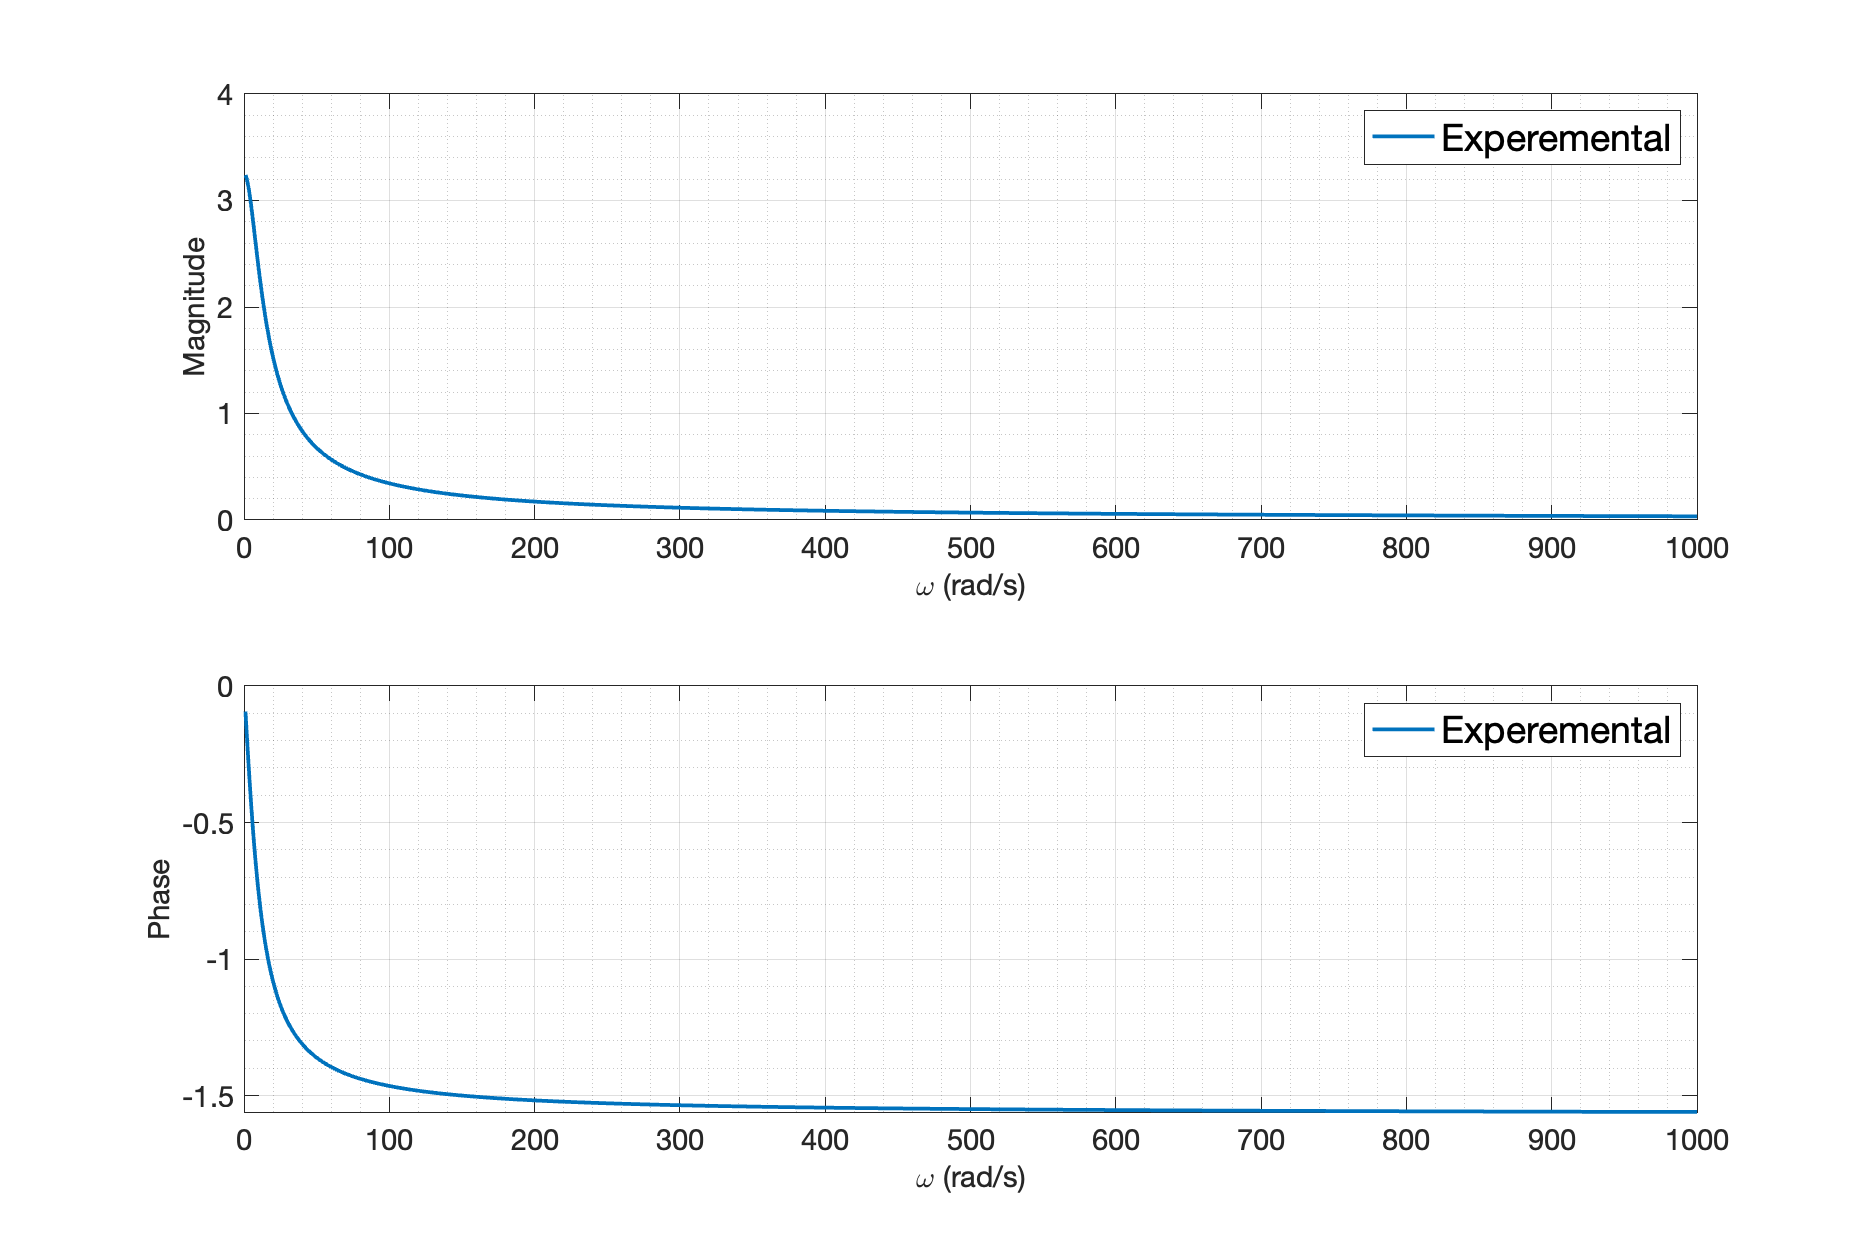
\includegraphics[width=\textwidth]{media/plots/task1_freq_resp_exp_lin.png}
    \caption{АЧХ и ФЧХ двигателя постоянного тока (экспериментально)}
    \label{fig:task1_freq_resp_exp_lin}
\end{figure}
\begin{figure}[ht!]
    \centering
    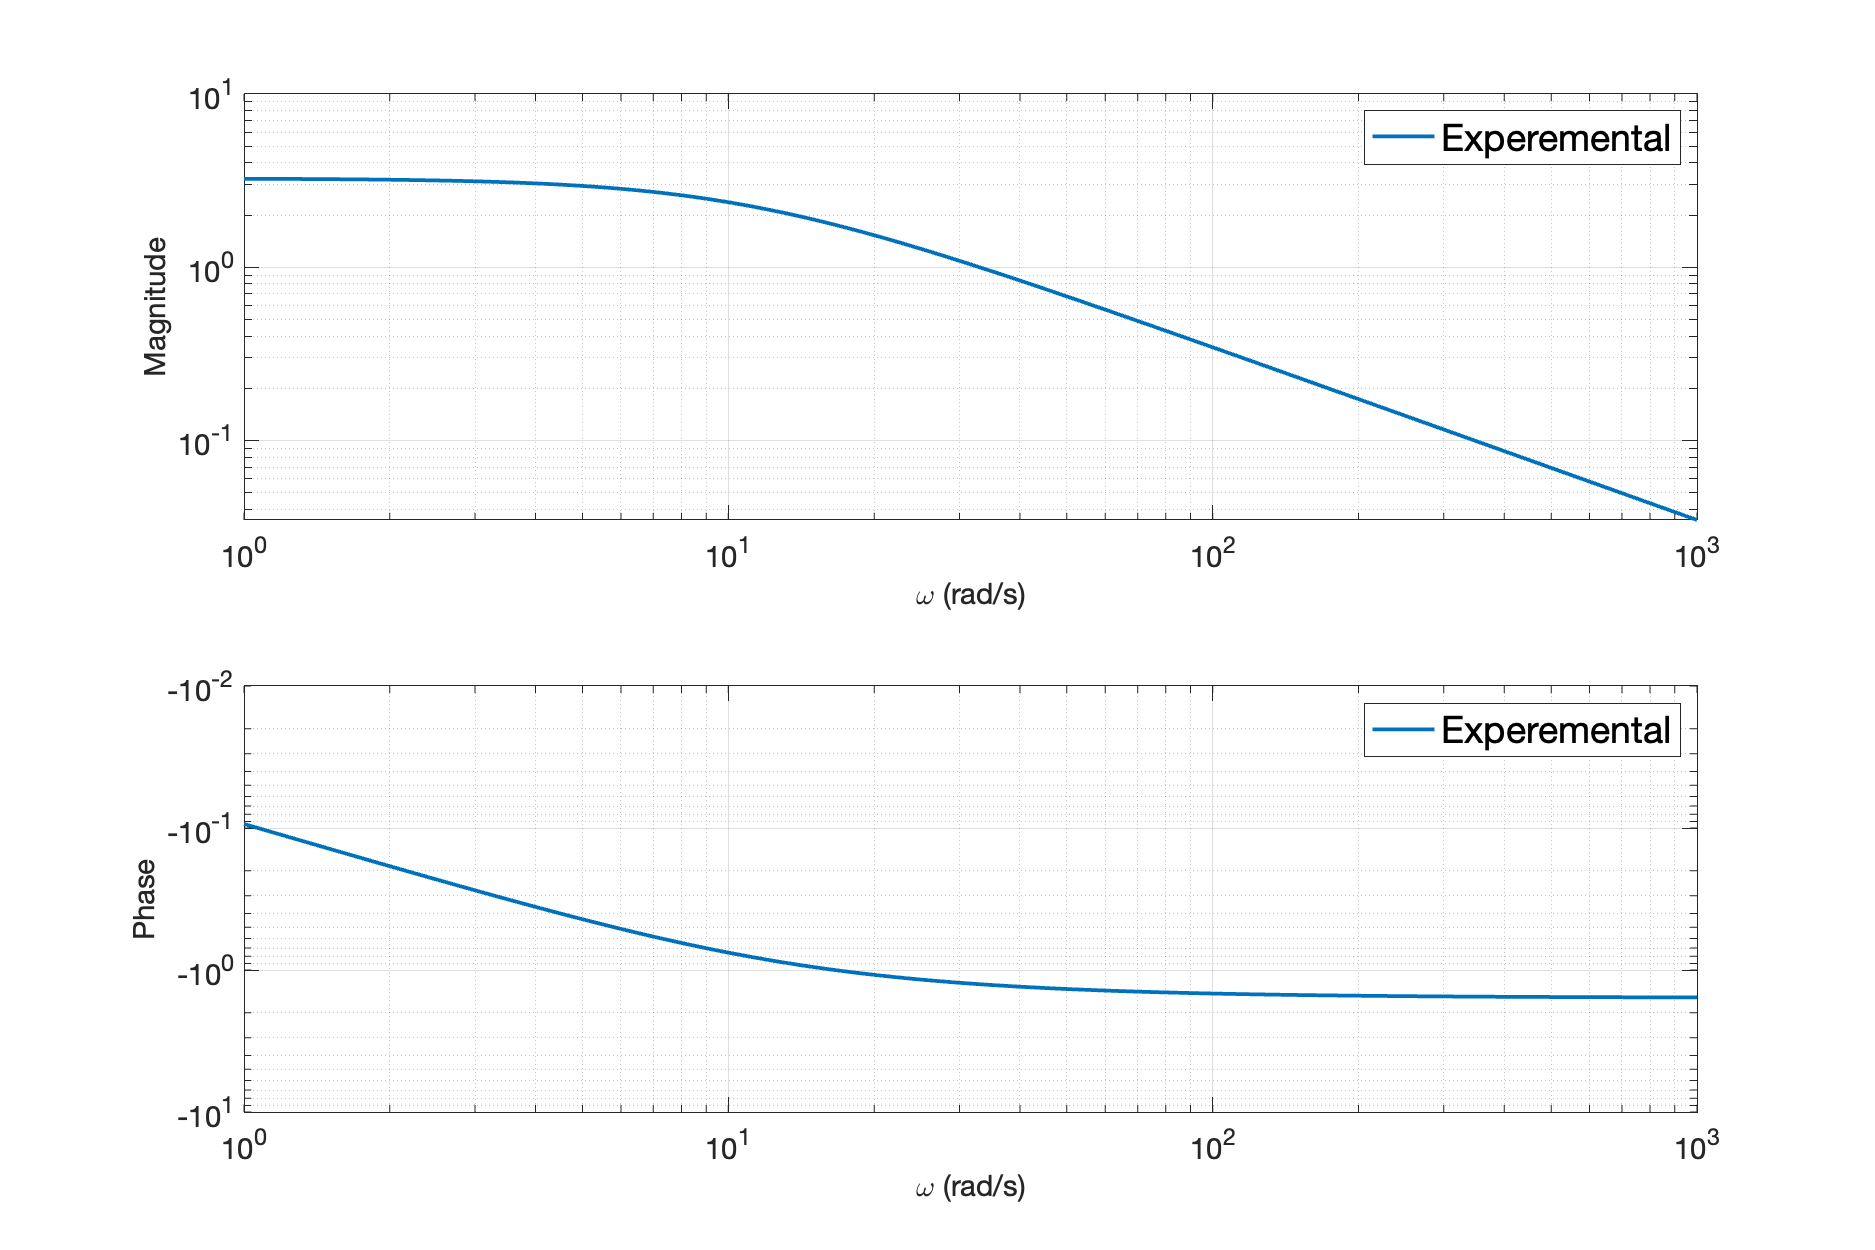
\includegraphics[width=\textwidth]{media/plots/task1_freq_resp_exp_loglog.png}
    \caption{Логарифмическая АЧХ двигателя постоянного тока (экспериментально)}
    \label{fig:task1_freq_resp_exp_loglog}
\end{figure}

Сравнительные графики приведены на рис. \ref{fig:task1_freq_resp_cmp_lin} и рис. \ref{fig:task1_freq_resp_cmp_loglog}.
\begin{figure}[ht!]
    \centering
    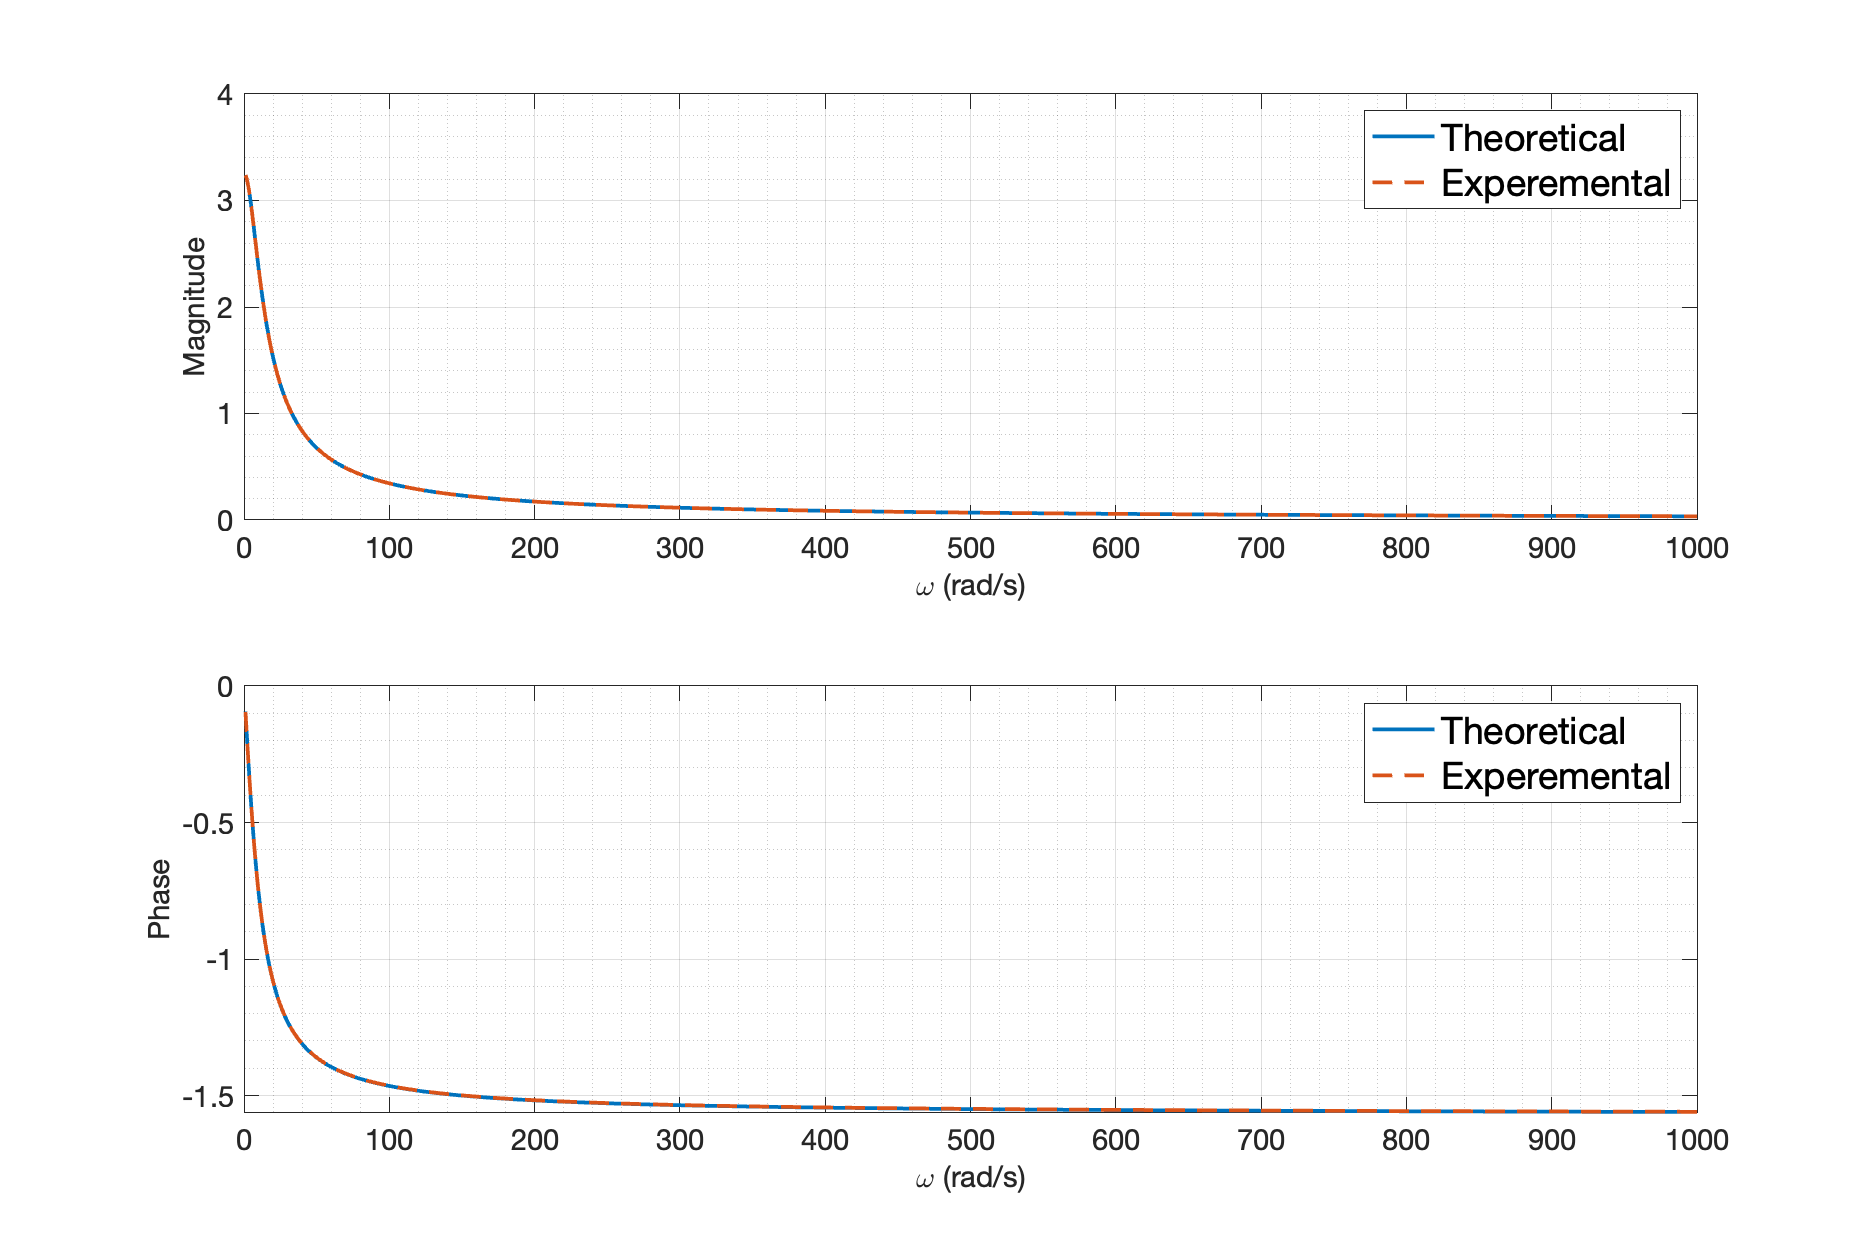
\includegraphics[width=\textwidth]{media/plots/task1_freq_resp_cmp_lin.png}
    \caption{Сравнение АЧХ и ФЧХ двигателя постоянного тока}
    \label{fig:task1_freq_resp_cmp_lin}
\end{figure}
\begin{figure}[ht!]
    \centering
    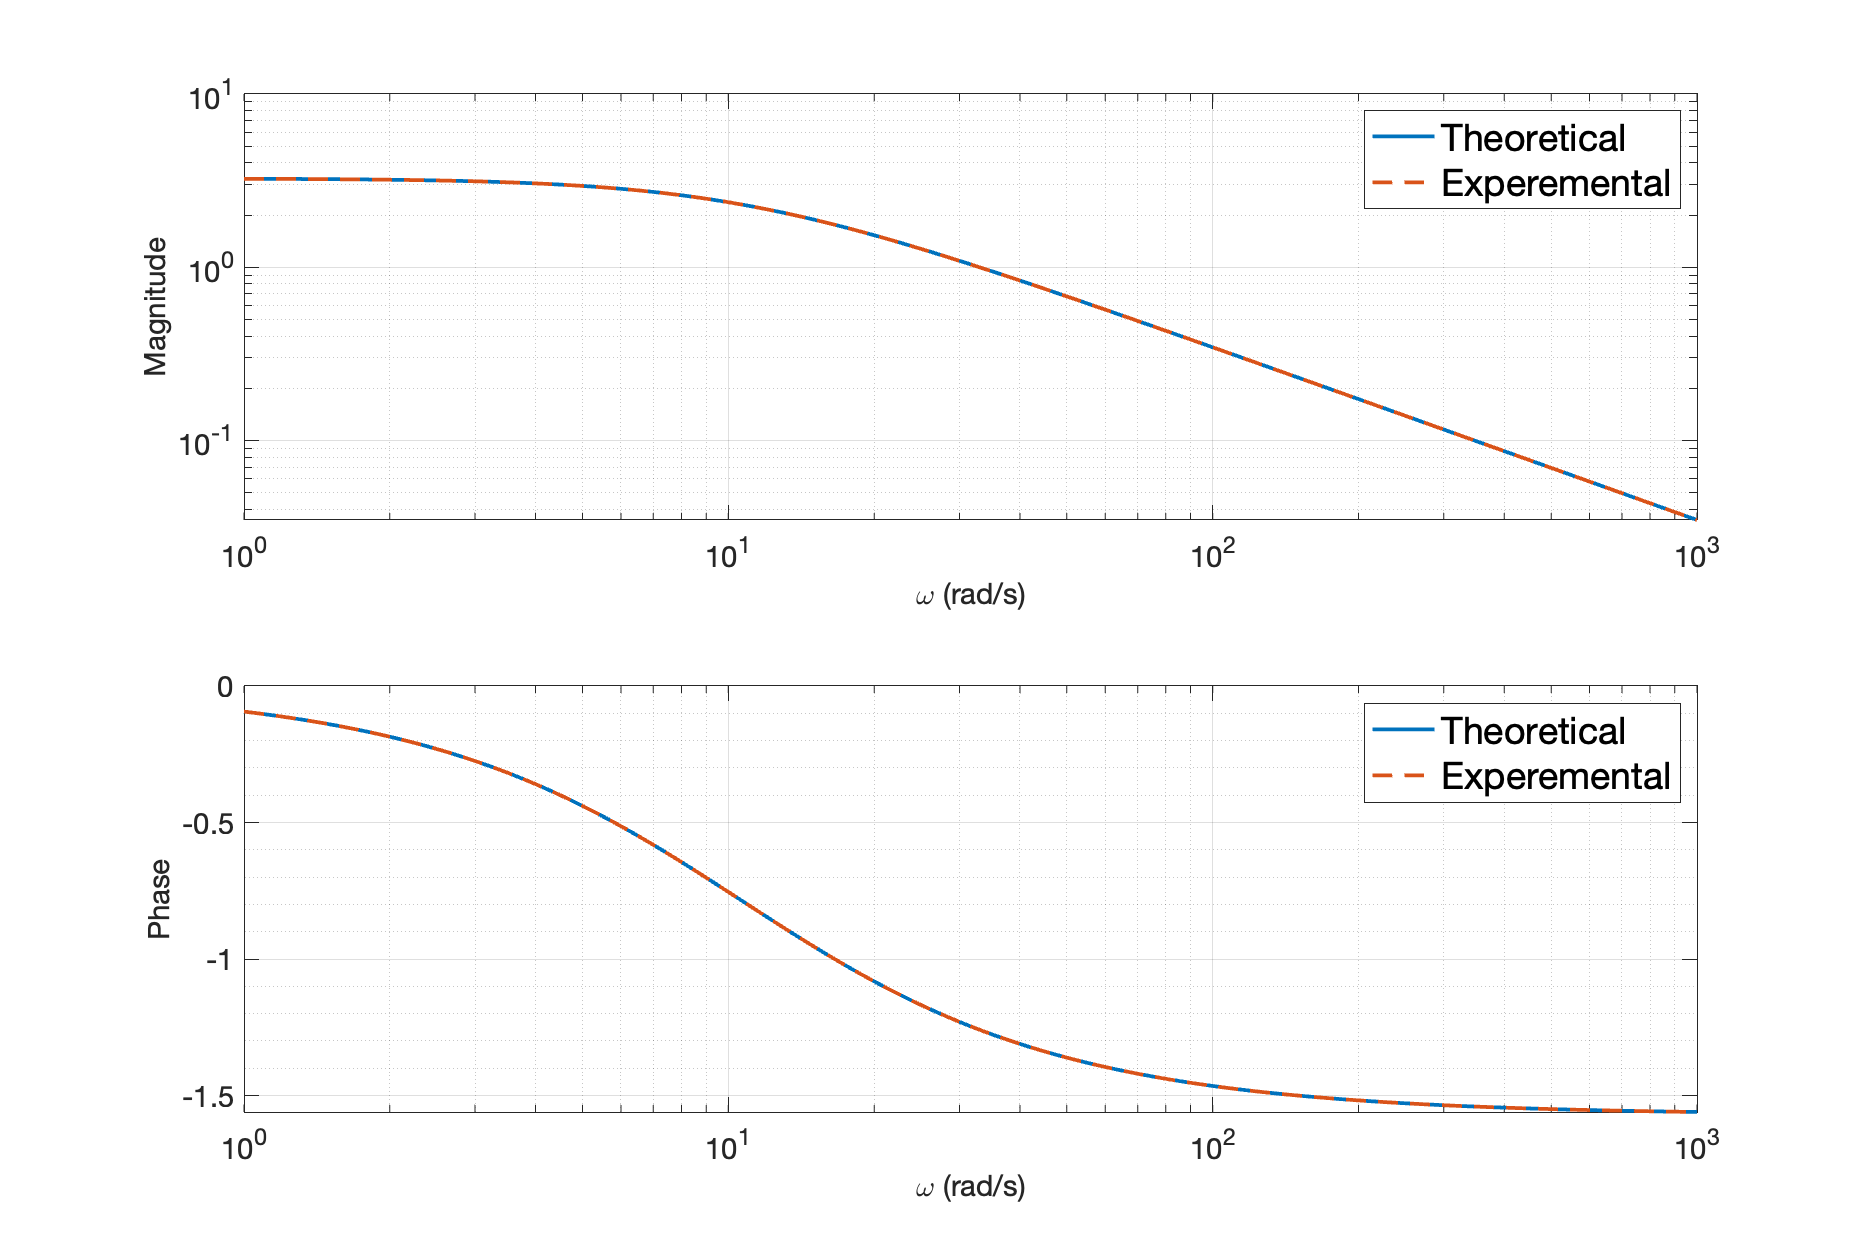
\includegraphics[width=\textwidth]{media/plots/task1_freq_resp_cmp_loglog.png}
    \caption{Сравнение логарифмической АЧХ двигателя постоянного тока}
    \label{fig:task1_freq_resp_cmp_loglog}
\end{figure}

Во всех случаях теоретические и экспериментальные графики совпадают, что 
говорит о корректности определения частотных характеристик. 